% Options for packages loaded elsewhere
\PassOptionsToPackage{unicode}{hyperref}
\PassOptionsToPackage{hyphens}{url}
%
\documentclass[
  ignorenonframetext,
]{beamer}
\usepackage{pgfpages}
\setbeamertemplate{caption}[numbered]
\setbeamertemplate{caption label separator}{: }
\setbeamercolor{caption name}{fg=normal text.fg}
\beamertemplatenavigationsymbolsempty
% Prevent slide breaks in the middle of a paragraph
\widowpenalties 1 10000
\raggedbottom
\setbeamertemplate{part page}{
  \centering
  \begin{beamercolorbox}[sep=16pt,center]{part title}
    \usebeamerfont{part title}\insertpart\par
  \end{beamercolorbox}
}
\setbeamertemplate{section page}{
  \centering
  \begin{beamercolorbox}[sep=12pt,center]{part title}
    \usebeamerfont{section title}\insertsection\par
  \end{beamercolorbox}
}
\setbeamertemplate{subsection page}{
  \centering
  \begin{beamercolorbox}[sep=8pt,center]{part title}
    \usebeamerfont{subsection title}\insertsubsection\par
  \end{beamercolorbox}
}
\AtBeginPart{
  \frame{\partpage}
}
\AtBeginSection{
  \ifbibliography
  \else
    \frame{\sectionpage}
  \fi
}
\AtBeginSubsection{
  \frame{\subsectionpage}
}

\usepackage{amsmath,amssymb}
\usepackage{iftex}
\ifPDFTeX
  \usepackage[T1]{fontenc}
  \usepackage[utf8]{inputenc}
  \usepackage{textcomp} % provide euro and other symbols
\else % if luatex or xetex
  \usepackage{unicode-math}
  \defaultfontfeatures{Scale=MatchLowercase}
  \defaultfontfeatures[\rmfamily]{Ligatures=TeX,Scale=1}
\fi
\usepackage{lmodern}
\usecolortheme{Flip}
\usefonttheme{serif} % use mainfont rather than sansfont for slide text
\useinnertheme{Flip}
\useoutertheme{Flip}
\ifPDFTeX\else  
    % xetex/luatex font selection
  \setmainfont[]{VisbyCF-Medium}
\fi
% Use upquote if available, for straight quotes in verbatim environments
\IfFileExists{upquote.sty}{\usepackage{upquote}}{}
\IfFileExists{microtype.sty}{% use microtype if available
  \usepackage[]{microtype}
  \UseMicrotypeSet[protrusion]{basicmath} % disable protrusion for tt fonts
}{}
\makeatletter
\@ifundefined{KOMAClassName}{% if non-KOMA class
  \IfFileExists{parskip.sty}{%
    \usepackage{parskip}
  }{% else
    \setlength{\parindent}{0pt}
    \setlength{\parskip}{6pt plus 2pt minus 1pt}}
}{% if KOMA class
  \KOMAoptions{parskip=half}}
\makeatother
\usepackage{xcolor}
\newif\ifbibliography
\setlength{\emergencystretch}{3em} % prevent overfull lines
\setcounter{secnumdepth}{-\maxdimen} % remove section numbering

\usepackage{color}
\usepackage{fancyvrb}
\newcommand{\VerbBar}{|}
\newcommand{\VERB}{\Verb[commandchars=\\\{\}]}
\DefineVerbatimEnvironment{Highlighting}{Verbatim}{commandchars=\\\{\}}
% Add ',fontsize=\small' for more characters per line
\usepackage{framed}
\definecolor{shadecolor}{RGB}{241,243,245}
\newenvironment{Shaded}{\begin{snugshade}}{\end{snugshade}}
\newcommand{\AlertTok}[1]{\textcolor[rgb]{0.68,0.00,0.00}{#1}}
\newcommand{\AnnotationTok}[1]{\textcolor[rgb]{0.37,0.37,0.37}{#1}}
\newcommand{\AttributeTok}[1]{\textcolor[rgb]{0.40,0.45,0.13}{#1}}
\newcommand{\BaseNTok}[1]{\textcolor[rgb]{0.68,0.00,0.00}{#1}}
\newcommand{\BuiltInTok}[1]{\textcolor[rgb]{0.00,0.23,0.31}{#1}}
\newcommand{\CharTok}[1]{\textcolor[rgb]{0.13,0.47,0.30}{#1}}
\newcommand{\CommentTok}[1]{\textcolor[rgb]{0.37,0.37,0.37}{#1}}
\newcommand{\CommentVarTok}[1]{\textcolor[rgb]{0.37,0.37,0.37}{\textit{#1}}}
\newcommand{\ConstantTok}[1]{\textcolor[rgb]{0.56,0.35,0.01}{#1}}
\newcommand{\ControlFlowTok}[1]{\textcolor[rgb]{0.00,0.23,0.31}{#1}}
\newcommand{\DataTypeTok}[1]{\textcolor[rgb]{0.68,0.00,0.00}{#1}}
\newcommand{\DecValTok}[1]{\textcolor[rgb]{0.68,0.00,0.00}{#1}}
\newcommand{\DocumentationTok}[1]{\textcolor[rgb]{0.37,0.37,0.37}{\textit{#1}}}
\newcommand{\ErrorTok}[1]{\textcolor[rgb]{0.68,0.00,0.00}{#1}}
\newcommand{\ExtensionTok}[1]{\textcolor[rgb]{0.00,0.23,0.31}{#1}}
\newcommand{\FloatTok}[1]{\textcolor[rgb]{0.68,0.00,0.00}{#1}}
\newcommand{\FunctionTok}[1]{\textcolor[rgb]{0.28,0.35,0.67}{#1}}
\newcommand{\ImportTok}[1]{\textcolor[rgb]{0.00,0.46,0.62}{#1}}
\newcommand{\InformationTok}[1]{\textcolor[rgb]{0.37,0.37,0.37}{#1}}
\newcommand{\KeywordTok}[1]{\textcolor[rgb]{0.00,0.23,0.31}{#1}}
\newcommand{\NormalTok}[1]{\textcolor[rgb]{0.00,0.23,0.31}{#1}}
\newcommand{\OperatorTok}[1]{\textcolor[rgb]{0.37,0.37,0.37}{#1}}
\newcommand{\OtherTok}[1]{\textcolor[rgb]{0.00,0.23,0.31}{#1}}
\newcommand{\PreprocessorTok}[1]{\textcolor[rgb]{0.68,0.00,0.00}{#1}}
\newcommand{\RegionMarkerTok}[1]{\textcolor[rgb]{0.00,0.23,0.31}{#1}}
\newcommand{\SpecialCharTok}[1]{\textcolor[rgb]{0.37,0.37,0.37}{#1}}
\newcommand{\SpecialStringTok}[1]{\textcolor[rgb]{0.13,0.47,0.30}{#1}}
\newcommand{\StringTok}[1]{\textcolor[rgb]{0.13,0.47,0.30}{#1}}
\newcommand{\VariableTok}[1]{\textcolor[rgb]{0.07,0.07,0.07}{#1}}
\newcommand{\VerbatimStringTok}[1]{\textcolor[rgb]{0.13,0.47,0.30}{#1}}
\newcommand{\WarningTok}[1]{\textcolor[rgb]{0.37,0.37,0.37}{\textit{#1}}}

\providecommand{\tightlist}{%
  \setlength{\itemsep}{0pt}\setlength{\parskip}{0pt}}\usepackage{longtable,booktabs,array}
\usepackage{calc} % for calculating minipage widths
\usepackage{caption}
% Make caption package work with longtable
\makeatletter
\def\fnum@table{\tablename~\thetable}
\makeatother
\usepackage{graphicx}
\makeatletter
\def\maxwidth{\ifdim\Gin@nat@width>\linewidth\linewidth\else\Gin@nat@width\fi}
\def\maxheight{\ifdim\Gin@nat@height>\textheight\textheight\else\Gin@nat@height\fi}
\makeatother
% Scale images if necessary, so that they will not overflow the page
% margins by default, and it is still possible to overwrite the defaults
% using explicit options in \includegraphics[width, height, ...]{}
\setkeys{Gin}{width=\maxwidth,height=\maxheight,keepaspectratio}
% Set default figure placement to htbp
\makeatletter
\def\fps@figure{htbp}
\makeatother

\usepackage{tabu}
\makeatletter
\makeatother
\makeatletter
\makeatother
\makeatletter
\@ifpackageloaded{caption}{}{\usepackage{caption}}
\AtBeginDocument{%
\ifdefined\contentsname
  \renewcommand*\contentsname{Table of contents}
\else
  \newcommand\contentsname{Table of contents}
\fi
\ifdefined\listfigurename
  \renewcommand*\listfigurename{List of Figures}
\else
  \newcommand\listfigurename{List of Figures}
\fi
\ifdefined\listtablename
  \renewcommand*\listtablename{List of Tables}
\else
  \newcommand\listtablename{List of Tables}
\fi
\ifdefined\figurename
  \renewcommand*\figurename{Figure}
\else
  \newcommand\figurename{Figure}
\fi
\ifdefined\tablename
  \renewcommand*\tablename{Table}
\else
  \newcommand\tablename{Table}
\fi
}
\@ifpackageloaded{float}{}{\usepackage{float}}
\floatstyle{ruled}
\@ifundefined{c@chapter}{\newfloat{codelisting}{h}{lop}}{\newfloat{codelisting}{h}{lop}[chapter]}
\floatname{codelisting}{Listing}
\newcommand*\listoflistings{\listof{codelisting}{List of Listings}}
\makeatother
\makeatletter
\@ifpackageloaded{caption}{}{\usepackage{caption}}
\@ifpackageloaded{subcaption}{}{\usepackage{subcaption}}
\makeatother
\makeatletter
\@ifpackageloaded{tcolorbox}{}{\usepackage[skins,breakable]{tcolorbox}}
\makeatother
\makeatletter
\@ifundefined{shadecolor}{\definecolor{shadecolor}{rgb}{.97, .97, .97}}
\makeatother
\makeatletter
\makeatother
\makeatletter
\makeatother
\ifLuaTeX
  \usepackage{selnolig}  % disable illegal ligatures
\fi
\IfFileExists{bookmark.sty}{\usepackage{bookmark}}{\usepackage{hyperref}}
\IfFileExists{xurl.sty}{\usepackage{xurl}}{} % add URL line breaks if available
\urlstyle{same} % disable monospaced font for URLs
\hypersetup{
  pdftitle={Réduction de la dimension},
  pdfauthor={Léo Belzile},
  hidelinks,
  pdfcreator={LaTeX via pandoc}}

\title{Réduction de la dimension}
\subtitle{Analyse multidimensionnelle appliquée}
\author{Léo Belzile}
\date{}
\institute{HEC Montréal}

\begin{document}
\frame{\titlepage}
\ifdefined\Shaded\renewenvironment{Shaded}{\begin{tcolorbox}[frame hidden, enhanced, sharp corners, borderline west={3pt}{0pt}{shadecolor}, interior hidden, breakable, boxrule=0pt]}{\end{tcolorbox}}\fi

\begin{frame}{Réduction de la dimension}
\protect\hypertarget{ruxe9duction-de-la-dimension}{}
On dispose de \(p\) variables explicatives \(X_1, \ldots, X_p\).

Comment réduire ce nombre de variables en conservant le plus
d'information possible?
\end{frame}

\begin{frame}{Analyse en composantes principales}
\protect\hypertarget{analyse-en-composantes-principales}{}
\begin{itemize}
\tightlist
\item
  maximiser la variabilité
\item
  créer de nouvelles variables non corrélées les unes avec les autres.
\end{itemize}
\end{frame}

\begin{frame}{Analyse factorielle exploratoire}
\protect\hypertarget{analyse-factorielle-exploratoire}{}
Utilisé principalement pour les questionnaires

\begin{itemize}
\tightlist
\item
  Trouver automatiquement des regroupements de variables
\item
  Créer des variables résumées (moyenne de variables)
\end{itemize}
\end{frame}

\begin{frame}{Coefficient de corrélation linéaire}
\protect\hypertarget{coefficient-de-corruxe9lation-linuxe9aire}{}
\begin{itemize}
\tightlist
\item
  Mesure la relation \emph{linéaire} entre variables
\item
  Valeur entre \(-1 \leq r \leq 1\).
\item
  Les points sont alignés (exactement) si \(r=\pm 1\); le signe
  détermine l'orientation de la pente.
\end{itemize}
\end{frame}

\begin{frame}{Datasaurus}
\protect\hypertarget{datasaurus}{}
\begin{figure}

{\centering 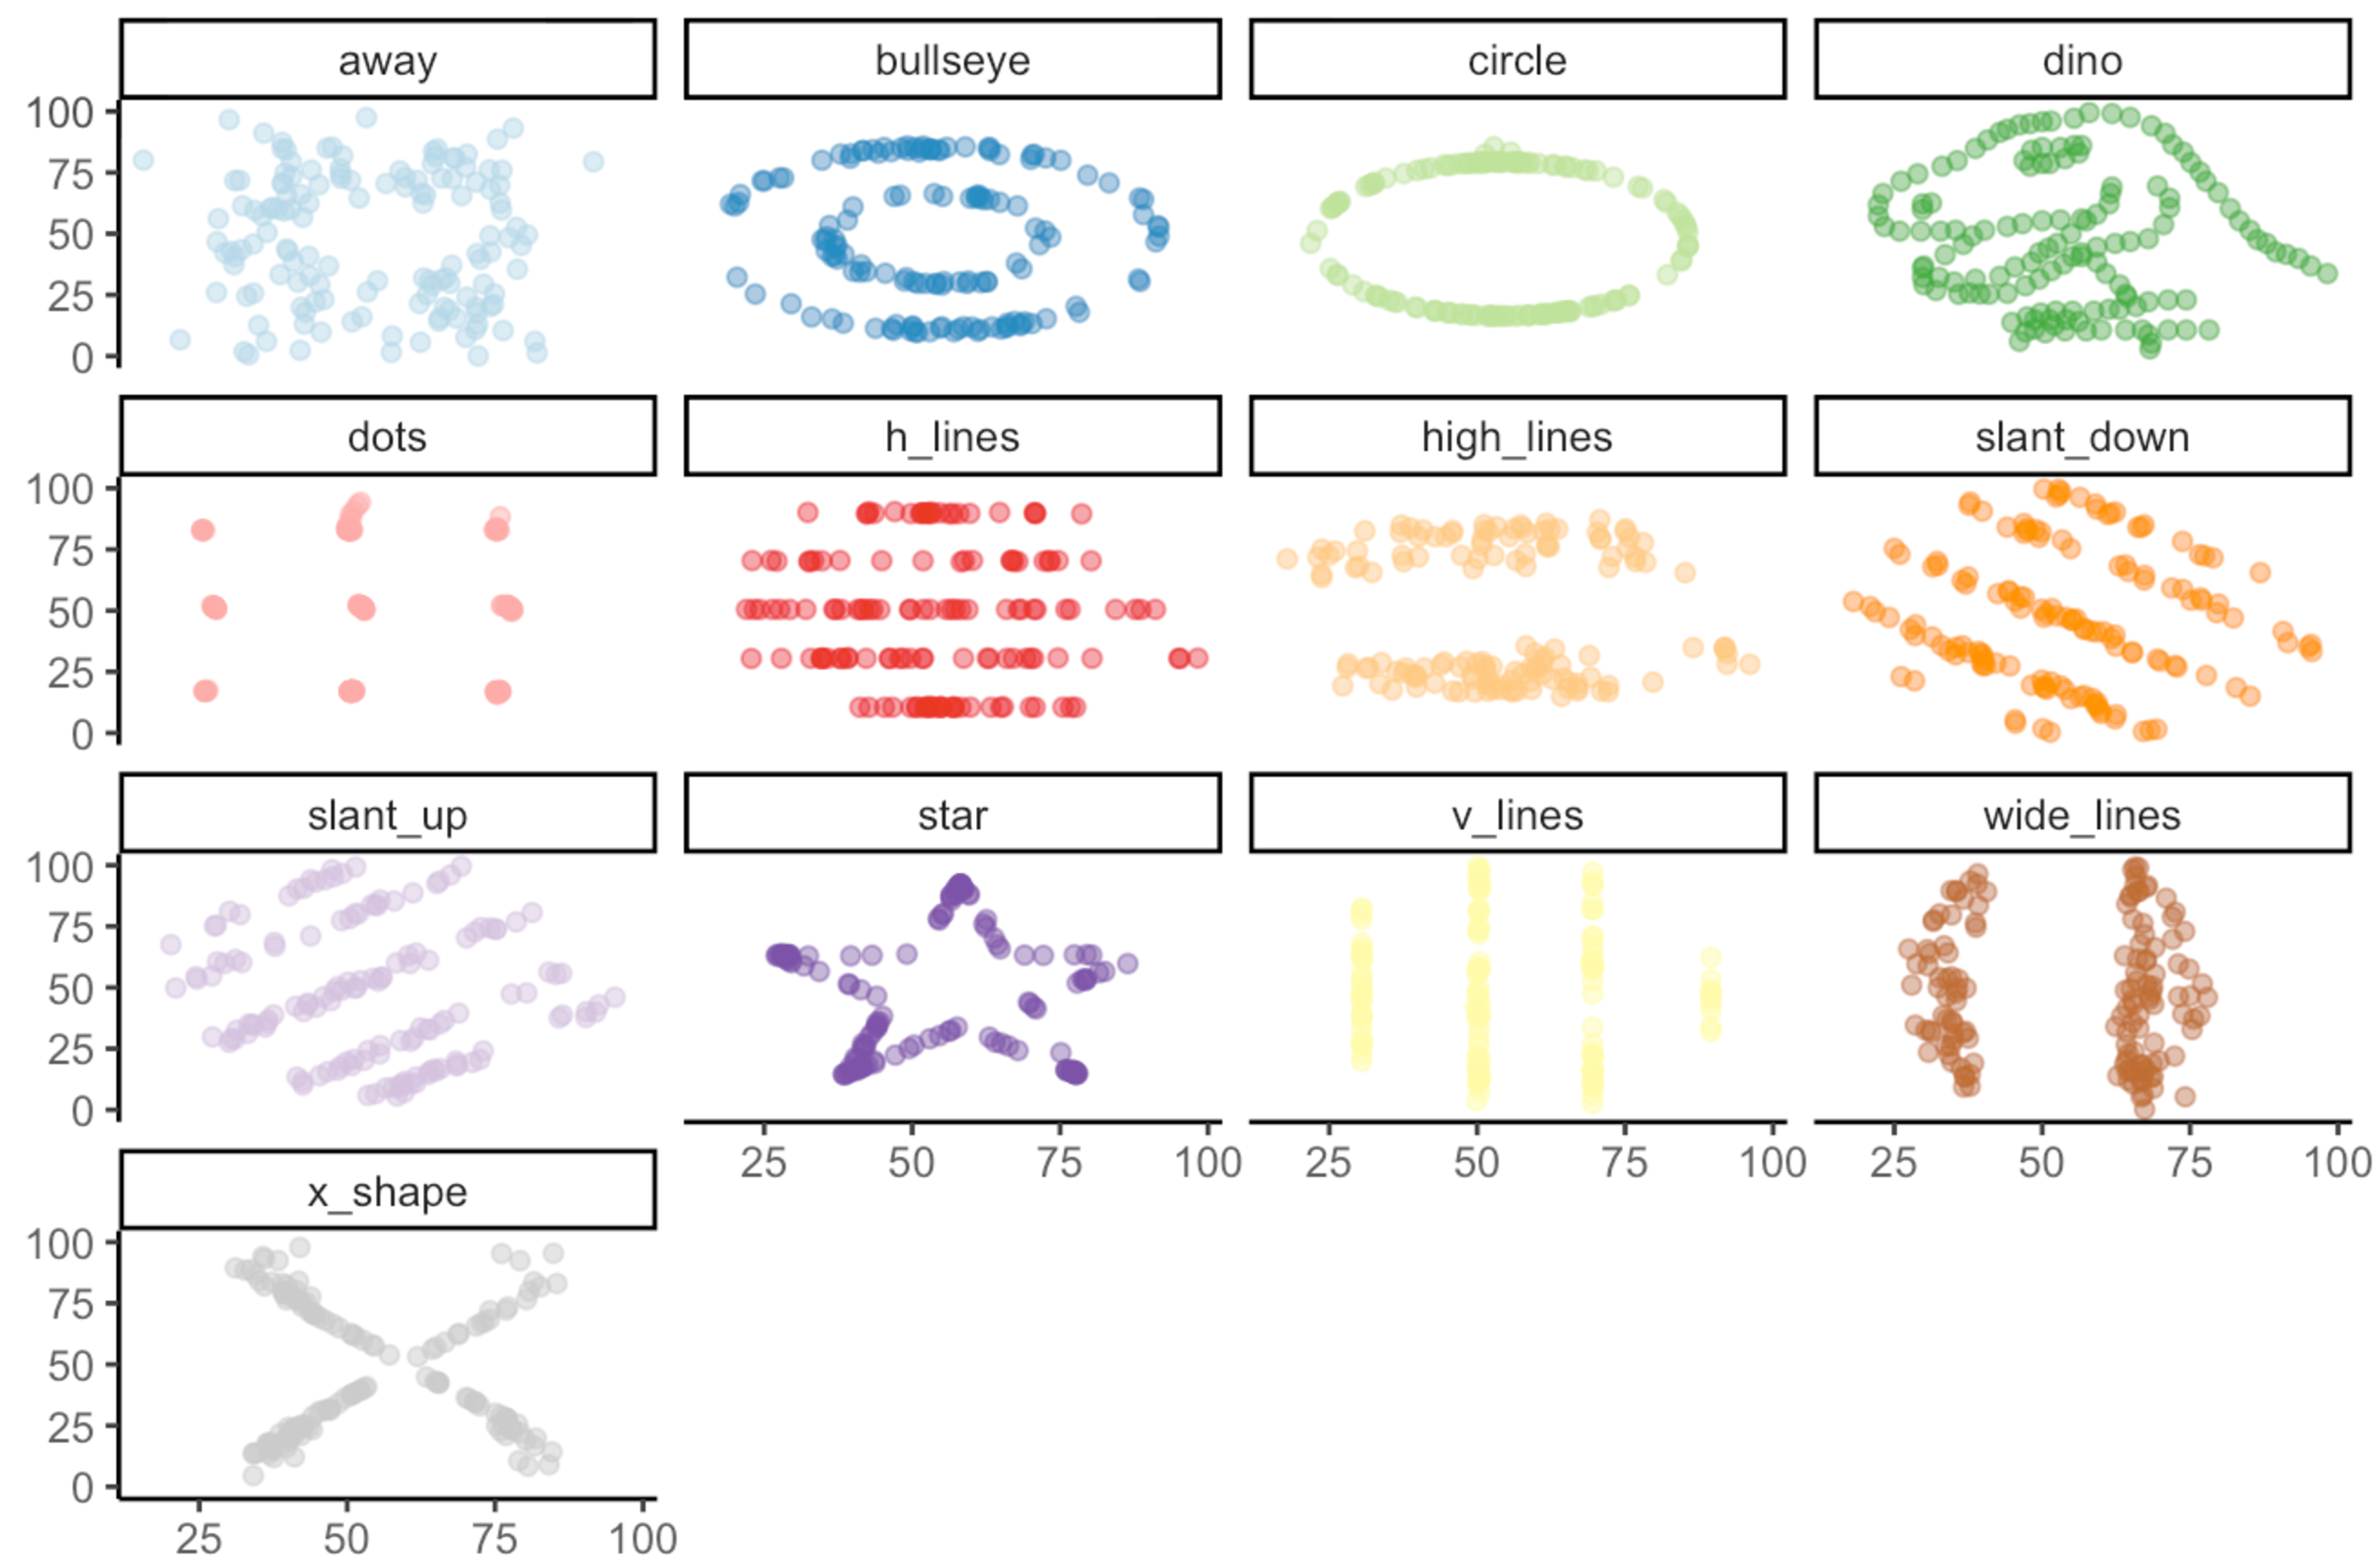
\includegraphics{figures/DataSaurusDozen.pdf}

}

\caption{Datasaurus (jeux de données avec la même corrélation)}

\end{figure}
\end{frame}

\begin{frame}{Exemple}
\protect\hypertarget{exemple}{}
\begin{itemize}
\tightlist
\item
  \textbf{Questions} sur une étude dans un magasin (200 répondants).
\item
  Réponses: échelles de Likert allant de pas important (1) à très
  important (5)
\end{itemize}

Pour vous, à quel point est-ce important

\scalebox{0.8}{
\begin{minipage}{\textwidth}

\begin{columns}[T]
\begin{column}{0.45\textwidth}
\begin{enumerate}
\tightlist
\item
  que le magasin offre de bons prix tous les jours?
\item
  que le magasin accepte les cartes de crédit majeures (Visa,
  Mastercard)?
\item
  que le magasin offre des produits de qualité?
\item
  que les vendeurs connaissent bien les produits?
\item
  qu'il y ait des ventes spéciales régulièrement?
\item
  que les marques connues soient disponibles?
\end{enumerate}
\end{column}

\begin{column}{0.45\textwidth}
\begin{enumerate}
\setcounter{enumi}{6}
\tightlist
\item
  que le magasin ait sa propre carte de crédit?
\item
  que le service soit rapide?
\item
  qu'il y ait une vaste sélection de produits?
\item
  que le magasin accepte le paiement par carte de débit?
\item
  que le personnel soit courtois?
\item
  que le magasin ait en stock les produits annoncés?
\end{enumerate}
\end{column}
\end{columns}

\end{minipage}
}
\end{frame}

\begin{frame}{Objectif des composantes principales}
\protect\hypertarget{objectif-des-composantes-principales}{}
Typiquement utilisé à des fins

\begin{itemize}
\tightlist
\item
  d'analyse exploratoire (visualisation) ou
\item
  pour créer une variable réponse (par ex., le quotient intellectuel)
\end{itemize}

Réduire la dimension en préservant le plus de variabilité possible.
\end{frame}

\begin{frame}{Composantes principales:}
\protect\hypertarget{composantes-principales}{}
\begin{itemize}
\tightlist
\item
  Créer des nouvelles variables \textbf{non corrélées} appelées
  \textbf{composantes principales} et dénotées \(C_1, \ldots, C_p\).
\item
  Les composantes principales sont des combinaisons linéaires des
  variables originales.
\end{itemize}

\begin{align*}
C_j &= \underset{\text{somme de poids fois variables explicatives}}{w_{j1} X_1 + w_{j2} X_2 + \cdots + w_{jp} X_p}, \qquad (j=1, \ldots, p),\\
1 &= \underset{\text{poids standardisés}}{w_{j1}^2 + \cdots + w_{jp}^2}
\end{align*}
\end{frame}

\begin{frame}[fragile]{Maximiser la variabilité}
\protect\hypertarget{maximiser-la-variabilituxe9}{}
\begin{align*}
\mathsf{Va}(C_1) \geq \cdots \geq \mathsf{Va}(C_p)
\end{align*} et \(\mathsf{Cor}(C_i, C_j)=0\) pour \(i \neq j\).

\begin{itemize}
\tightlist
\item
  L'ensemble de \(k\) variables qui maximise la variance totale exprimée
  est \(C_1, \ldots, C_k\).
\item
  Par construction, la variance des composantes principales est
  décroissante.
\end{itemize}

\hypertarget{tbl-eigenvalues}{}
\begin{table}
\caption{\label{tbl-eigenvalues}Variance des premières composantes principales }\tabularnewline

\centering
\begin{tabular}[t]{cccccccc}
\toprule
C1 & C2 & C3 & C4 & C5 & C6 & C7 & C8\\
\midrule
2.43 & 2.00 & 1.94 & 1.30 & 0.74 & 0.69 & 0.57 & 0.54\\
\bottomrule
\end{tabular}
\end{table}
\end{frame}

\begin{frame}{Calcul des composantes principales}
\protect\hypertarget{calcul-des-composantes-principales}{}
On calcule la matrice de covariance (ou de corrélation) et on effectue
une décomposition en valeurs propres/vecteurs propres.

\begin{itemize}
\tightlist
\item
  Les valeurs propres donnent les variances des différentes composantes.
\item
  Les vecteurs propres donnent la matrice de changement de base pour
  obtenir les composantes principales.
\item
  Les vecteurs propres (et donc les composantes) sont orthogonales
\end{itemize}
\end{frame}

\begin{frame}[fragile]{Calcul dans \textbf{R}}
\protect\hypertarget{calcul-dans-r}{}
\begin{Shaded}
\begin{Highlighting}[]
\NormalTok{mat\_cor }\OtherTok{\textless{}{-}} \FunctionTok{cor}\NormalTok{(factor)}
\NormalTok{decompo }\OtherTok{\textless{}{-}} \FunctionTok{eigen}\NormalTok{(mat\_cor)}
\CommentTok{\# Variances des composantes principales}
\NormalTok{variances }\OtherTok{\textless{}{-}}\NormalTok{ decompo}\SpecialCharTok{$}\NormalTok{values}
\CommentTok{\# Il faut standardiser les données}
\NormalTok{factor\_std }\OtherTok{\textless{}{-}} \FunctionTok{as.matrix}\NormalTok{(}\FunctionTok{scale}\NormalTok{(factor))}
\NormalTok{composantes }\OtherTok{\textless{}{-}}\NormalTok{ factor\_std }\SpecialCharTok{\%*\%}\NormalTok{ decompo}\SpecialCharTok{$}\NormalTok{vectors}
\CommentTok{\# cor(composantes) \# corrélations nulles}
\end{Highlighting}
\end{Shaded}
\end{frame}

\begin{frame}{Covariance ou corrélation?}
\protect\hypertarget{covariance-ou-corruxe9lation}{}
La matrice de corrélation est la matrice de covariance des données
\textbf{standardisées} (variance unitaire)

\begin{itemize}
\tightlist
\item
  la covariance accorde plus d'importante aux variables qui ont une
  variance élevée
\item
  si les variables sont sur la même échelle, covariance et corrélation
  sont utilisables
\item
  sinon, utiliser la matrice de corrélation \emph{par défaut}.
\end{itemize}
\end{frame}

\begin{frame}{Rotation et système de coordonnées}
\protect\hypertarget{rotation-et-systuxe8me-de-coordonnuxe9es}{}
\begin{figure}

{\centering \includegraphics[width=0.9\textwidth,height=\textheight]{MATH60602-diapos10_files/figure-beamer/fig-acprotation-1.pdf}

}

\caption{\label{fig-acprotation}Nuage de points avant (gauche) et après
(droite) analyse en composantes principales.}

\end{figure}
\end{frame}

\begin{frame}[fragile]{Implémentation en \textbf{R}}
\protect\hypertarget{impluxe9mentation-en-r}{}
\begin{Shaded}
\begin{Highlighting}[]
\CommentTok{\# Analyse en composantes principales}
\CommentTok{\# de la matrice de corrélation}
\NormalTok{acp }\OtherTok{\textless{}{-}} \FunctionTok{princomp}\NormalTok{(factor, }\AttributeTok{cor =} \ConstantTok{TRUE}\NormalTok{)}
\FunctionTok{biplot}\NormalTok{(acp) }\CommentTok{\# bigramme}
\end{Highlighting}
\end{Shaded}
\end{frame}

\begin{frame}{Matrice de chargements}
\protect\hypertarget{matrice-de-chargements}{}
\footnotesize

\begin{table}
\centering
\begin{tabular}{lllllllll}
\toprule
  & C1 & C2 & C3 & C4 & C5 & C6 & C7 & C8\\
\midrule
x1 & 0.21 &  &  & 0.65 & 0.27 & 0.41 & 0.45 & \\
x2 &  &  & -0.53 &  &  & 0.24 & -0.3 & 0.41\\
x3 & -0.39 & 0.36 &  &  & -0.21 &  &  & -0.26\\
x4 & -0.36 & -0.34 & 0.25 &  &  &  &  & 0.25\\
x5 &  &  &  & 0.69 & -0.32 & -0.36 & -0.46 & \\
\addlinespace
x6 & -0.29 & 0.34 &  &  & 0.74 & -0.41 &  & \\
x7 & -0.23 &  & -0.51 &  &  &  &  & \\
x8 & -0.35 & -0.4 & 0.21 &  &  &  &  & \\
x9 & -0.28 & 0.42 &  &  & -0.4 &  & 0.42 & 0.51\\
x10 & -0.27 &  & -0.45 &  &  &  & 0.44 & -0.56\\
\addlinespace
x11 & -0.31 & -0.34 & 0.35 &  &  &  &  & \\
x12 & -0.33 & 0.36 &  &  &  & 0.63 & -0.31 & -0.28\\
\bottomrule
\end{tabular}
\end{table}

\footnotesize

Tableau des poids \(\mathbf{W}\). Les poids inférieurs à 0.2 en valeur
absolue sont omis.
\end{frame}

\begin{frame}{Bigramme}
\protect\hypertarget{bigramme}{}
\begin{figure}

{\centering \includegraphics[width=0.7\textwidth,height=\textheight]{MATH60602-diapos10_files/figure-beamer/fig-bigramme-1.pdf}

}

\caption{\label{fig-bigramme}Bigramme (représentation sur les deux
premières composantes principales)}

\end{figure}
\end{frame}

\begin{frame}{Interprétation du bigramme}
\protect\hypertarget{interpruxe9tation-du-bigramme}{}
\begin{itemize}
\tightlist
\item
  Le nuage de points représente les nouvelles coordonnées des \(n\)
  observations dans l'espace engendré par les deux premières composantes
  principales.
\item
  Les flèches donnent les poids de chaque variable servant à la création
  des composantes (ces poids sont appelés chargements).
\item
  On peut distinguer des directions générales qui représentent
  l'orientation: si des variables pointent dans la même direction, elles
  sont typiquement fortement corrélées.
\end{itemize}
\end{frame}

\begin{frame}[fragile]{Choix du nombre de composantes}
\protect\hypertarget{choix-du-nombre-de-composantes}{}
L'objectif est de réduire la dimension, on ne conserve qu'une poignée de
composantes.

\begin{itemize}
\tightlist
\item
  \textbf{critère des valeurs propres de Kaiser}: variances des
  composantes principales (valeurs propres) supérieures à 1.
\item
  \textbf{critère du coude de Cattell}: diagramme d'éboulis
  (\texttt{screeplot})
\end{itemize}

\begin{Shaded}
\begin{Highlighting}[]
\NormalTok{hecmulti}\SpecialCharTok{::}\FunctionTok{eboulis}\NormalTok{(acp)}
\end{Highlighting}
\end{Shaded}
\end{frame}

\begin{frame}{Diagramme d'éboulis}
\protect\hypertarget{diagramme-duxe9boulis}{}
\begin{figure}

{\centering \includegraphics[width=0.7\textwidth,height=\textheight]{MATH60602-diapos10_files/figure-beamer/fig-screeplot-1.pdf}

}

\caption{\label{fig-screeplot}Diagramme d'éboulis (gauche) et variance
cumulative (droite).}

\end{figure}
\end{frame}

\begin{frame}{Pourcentage de variance exprimée}
\protect\hypertarget{pourcentage-de-variance-exprimuxe9e}{}
La variance totale des composantes principales est identique à celle des
variables originales:
\[\mathsf{Va}(C_1) + \cdots + \mathsf{Va}(C_p) = \mathsf{Va}(X_1) + \cdots + \mathsf{Va}(X_p)\]

\begin{itemize}
\tightlist
\item
  Si on travaille avec la matrice de corrélation (variance unitaire),
  alors la variance totale est \(p\).
\end{itemize}
\end{frame}

\begin{frame}{Inconvénients des composantes principales}
\protect\hypertarget{inconvuxe9nients-des-composantes-principales}{}
\begin{itemize}
\tightlist
\item
  Toutes les variables sont nécessaires pour créer des composantes
  principales avec de nouvelles observations
\item
  Le critère d'optimisation ne prend pas en compte une potentielle
  variable réponse. Dans chaque cas, on cherche une combinaison linéaire
  des variables explicatives telle que

  \begin{itemize}
  \tightlist
  \item
    la variance de cette combinaison est maximale (ACP)
  \item
    la corrélation avec \(Y\) est maximale (analyse canonique)
  \item
    la covariance avec \(Y\) est maximale (moindres carrés partiels,
    PLS).
  \end{itemize}
\end{itemize}
\end{frame}

\begin{frame}{Motivation pour l'analyse factorielle}
\protect\hypertarget{motivation-pour-lanalyse-factorielle}{}
\begin{itemize}
\tightlist
\item
  Y a-t-il des groupements de variables?
\item
  Est-ce que les variables faisant partie d'un groupement semblent
  mesurer certains aspects d'un facteur commun (non observé)?
\end{itemize}

De tels groupements peuvent être détectés (automatiquement) si plusieurs
variables sont très corrélées entre elles.
\end{frame}

\begin{frame}
\begin{figure}

{\centering \includegraphics[width=0.8\textwidth,height=\textheight]{MATH60602-diapos10_files/figure-beamer/fig-correlogram-1.pdf}

}

\caption{\label{fig-correlogram}Corrélogramme des items du
questionnaire}

\end{figure}
\end{frame}

\begin{frame}{Analyse factorielle exploratoire}
\protect\hypertarget{analyse-factorielle-exploratoire-1}{}
On possède \(n\) observations sur \(p\) variables et on s'intéresse à la
matrice de covariance (corrélation) qui décrit la relation linéaire.

Avec \(np\) données, on cherche à estimer \(p\) paramètres de variances
et \(p(p-1)/2\) corrélations.

On cherche un modèle plus \textbf{parcimonieux} pour expliquer la
dépendances.
\end{frame}

\begin{frame}{Facteurs}
\protect\hypertarget{facteurs}{}
On suppose qu'il existe \(m < p\) \textbf{facteurs} latents
\(F_1, \ldots, F_m\) qui suffisent à expliquer les variables
explicatives

Les facteurs sont:

\begin{itemize}
\tightlist
\item
  des variables aléatoires non observables
\item
  non corrélées entre elles
\item
  standardisées de moyenne zéro et variance unitaire.
\end{itemize}
\end{frame}

\begin{frame}{Modèle d'analyse factorielle (corrélation)}
\protect\hypertarget{moduxe8le-danalyse-factorielle-corruxe9lation}{}
Soit \(X_1, \ldots, X_p\) des variables explicatives
\emph{standardisées} (moyenne nulle, variance unitaire).

Cela revient à travailler avec la matrice de corrélation

\begin{align*}
X_j = \underset{\text{combinaison linéaire pondérée des facteurs}}{\gamma_{j1}F_1 + \cdots + \gamma_{jm}F_m} + \underset{\text{aléa}}{\varepsilon_j},\qquad j=1, \ldots, p.
\end{align*} où \(\varepsilon_j\) est un aléa de variance \(\psi_j\) et
de moyenne nulle.
\end{frame}

\begin{frame}{Chargements}
\protect\hypertarget{chargements}{}
\begin{align*}
X_j = \underset{\text{combinaison linéaire pondérée des facteurs}}{\gamma_{j1}F_1 + \cdots + \gamma_{jm}F_m} + \underset{\text{aléa}}{\varepsilon_j}, \qquad j=1, \ldots, p.
\end{align*}

Le chargement \(\gamma_{ij}\) mesure la corrélation entre \(X_i\) et
\(F_j\), \begin{align*}
\gamma_{ij} = \mathsf{Cor}(X_i, F_j).
\end{align*}

La proportion de la variance de \(X_i\) expliquée par les facteurs est
\(\gamma_{i1}^2 + \cdots + \gamma_{im}^2\).
\end{frame}

\begin{frame}{Exemple d'estimation des chargements}
\protect\hypertarget{exemple-destimation-des-chargements}{}
\hypertarget{tbl-factocp}{}
\begin{table}
\caption{\label{tbl-factocp}Estimés des chargements (pourcentage). }\tabularnewline

\centering
\begin{tabular}{lrrrr}
\toprule
  & F1 & F2 & F3 & F4\\
\midrule
x1 &  &  &  & 81\\
x2 &  &  & -79 & \\
x3 & 79 &  &  & \\
x4 &  & 82 &  & \\
x5 &  &  &  & 83\\
\addlinespace
x6 & 66 &  &  & \\
x7 &  &  & -83 & \\
x8 &  & 85 &  & \\
x9 & 75 &  &  & \\
x10 &  &  & -79 & \\
\addlinespace
x11 &  & 82 &  & \\
x12 & 73 &  &  & \\
\bottomrule
\end{tabular}
\end{table}

:::
\end{frame}

\begin{frame}{Analyse factorielle en pratique}
\protect\hypertarget{analyse-factorielle-en-pratique}{}
La corrélation entre les variables explicatives découlera de celle avec
les facteurs

Le modèle factorielle donne une approximation de la corrélation.
\end{frame}

\begin{frame}{Combien d'observations pour l'estimation?}
\protect\hypertarget{combien-dobservations-pour-lestimation}{}
Il faut un échantillon de taille conséquente.

\begin{itemize}
\tightlist
\item
  entre 5 et 20 fois \(p\), le nombre de variables
\item
  un nombre minimal de \(n=100\) à \(n=1000\) observations
\end{itemize}

Essentiellement des règles du pouce.
\end{frame}

\begin{frame}{Invariance aux rotations orthogonales}
\protect\hypertarget{invariance-aux-rotations-orthogonales}{}
On transforme la solution pour garantir une solution
\textbf{interprétable} puisque cette dernière n'est pas unique.

\begin{itemize}
\tightlist
\item
  La rotation \emph{varimax} maximise la variance de la somme des carrés
  des chargements pour les facteurs.
\item
  Donne des chargements dispersés (valeurs élevées positives ou
  négatives, d'autres presque nuls).
\end{itemize}
\end{frame}

\begin{frame}{Chargements après rotation varimax}
\protect\hypertarget{chargements-apruxe8s-rotation-varimax}{}
\begin{figure}

{\centering \includegraphics[width=0.7\textwidth,height=\textheight]{MATH60602-diapos10_files/figure-beamer/unnamed-chunk-11-1.pdf}

}

\end{figure}
\end{frame}

\begin{frame}[fragile]{Estimation avec composantes principales}
\protect\hypertarget{estimation-avec-composantes-principales}{}
Garder \(m\) vecteurs propres et valeurs propres, puis effectuer une
rotation (varimax)

\begin{itemize}
\tightlist
\item
  estimation toujours valide et rapide.
\item
  sélection moins objective que maximum de vraisemblance (critère du
  coude ou de Kaiser)
\end{itemize}

\begin{Shaded}
\begin{Highlighting}[]
\FunctionTok{library}\NormalTok{(hecmulti)}
\NormalTok{facto\_cp }\OtherTok{\textless{}{-}} \FunctionTok{factocp}\NormalTok{(factor, }
                    \AttributeTok{nfact =} \StringTok{"kaiser"}\NormalTok{, }
                    \AttributeTok{cor =} \ConstantTok{TRUE}\NormalTok{)}
\CommentTok{\# nfact: nombre de facteurs ("kaiser" par défaut)}
\CommentTok{\# cor: matrice de corrélation? par défaut vrai}
\end{Highlighting}
\end{Shaded}
\end{frame}

\begin{frame}{Estimation par maximum de vraisemblance}
\protect\hypertarget{estimation-par-maximum-de-vraisemblance}{}
\begin{itemize}
\tightlist
\item
  Postulat de normalité des aléas et des facteurs.
\item
  Nécessite une optimisation numérique délicate:

  \begin{itemize}
  \tightlist
  \item
    les problèmes de convergence sont fréquents
  \item
    variances estimées parfois négatives!
  \item
    appelés cas de \textbf{(quasi)-Heywood}.
  \end{itemize}
\item
  Méthodes de sélection plus informatives

  \begin{itemize}
  \tightlist
  \item
    critères d'information
  \item
    tests d'hypothèse d'adéquation
  \end{itemize}
\end{itemize}
\end{frame}

\begin{frame}{Choix du nombre de facteurs}
\protect\hypertarget{choix-du-nombre-de-facteurs}{}
Plus le nombre de facteurs \(m\) est grand, plus la corrélation
modélisée se rapproche de la corrélation empirique.

Mais plus le nombre de paramètres est grand\ldots{}
\end{frame}

\begin{frame}{Critères d'information}
\protect\hypertarget{crituxe8res-dinformation}{}
Valable uniquement pour les modèles ajustés par \textbf{maximum de
vraisemblance}

\begin{align*}
\mathsf{AIC} &= -\text{ajustement} + 2\times\text{nb param} \\
\mathsf{BIC}&= -\text{ajustement} + \ln(n)\times\text{nb param}
\end{align*}

\begin{itemize}
\tightlist
\item
  Plus le critère d'information est petit, meilleur c'est
\item
  Le \(\mathsf{BIC}\) (critère Bayésien de Schwarz) pénalise davantage
  que le \(\mathsf{AIC}\) (critère d'Akaike).
\end{itemize}
\end{frame}

\begin{frame}[fragile]{Choix du nombre de critères}
\protect\hypertarget{choix-du-nombre-de-crituxe8res}{}
\begin{Shaded}
\begin{Highlighting}[]
\FunctionTok{library}\NormalTok{(hecmulti)}
\FunctionTok{ajustement\_factanal}\NormalTok{(}
    \AttributeTok{covmat =} \FunctionTok{cor}\NormalTok{(factor), }\CommentTok{\# matrice de corrélation}
    \AttributeTok{factors =} \DecValTok{1}\SpecialCharTok{:}\DecValTok{5}\NormalTok{, }\CommentTok{\# candidats pour nb de facteurs}
    \AttributeTok{n.obs =} \FunctionTok{nrow}\NormalTok{(factor)) }\CommentTok{\# nombre d\textquotesingle{}observations}
\end{Highlighting}
\end{Shaded}
\end{frame}

\begin{frame}{Tableau résumé pour nombre de critères}
\protect\hypertarget{tableau-ruxe9sumuxe9-pour-nombre-de-crituxe8res}{}
\hypertarget{tbl-emvcrit}{}
\begin{table}
\caption{\label{tbl-emvcrit}Qualité de l'ajustement de modèles d'analyse factorielle (maximum de
vraisemblance). }\tabularnewline

\centering
\begin{tabular}{rrrlrr}
\toprule
k & AIC & BIC & valeur-p & npar & heywood\\
\midrule
1 & 2267.14 & 2346.30 & < 2e-16 & 24 & 0\\
2 & 2137.87 & 2253.31 & < 2e-16 & 35 & 0\\
3 & 2017.19 & 2165.61 & 0.09604 & 45 & 0\\
4 & 2002.56 & 2180.67 & 0.97262 & 54 & 1\\
5 & 2012.70 & 2217.19 & 0.97445 & 62 & 1\\
\bottomrule
\end{tabular}
\end{table}
\end{frame}

\begin{frame}{Résumé}
\protect\hypertarget{ruxe9sumuxe9}{}
Le tableau inclut

\begin{itemize}
\item
  critères d'informations AIC et BIC
\item
  valeur-\emph{p} du test de rapport de vraisemblance comparant le
  modèle saturé (corrélation empirique) et le modèle factoriel
\item
  nombre de paramètres estimés
\item
  indicateur pour les cas de (quasi)-Heywood
\end{itemize}
\end{frame}

\begin{frame}[fragile]{Ajustement}
\protect\hypertarget{ajustement}{}
Les critères d'information suggèrent \(m=4\) facteurs (\(\mathsf{AIC}\))
ou \(m=3\) (\(\mathsf{BIC}\))

\begin{itemize}
\tightlist
\item
  mais la solution à quatre facteurs n'est pas valide.
\item
  le modèle à trois facteurs est préférable (simplification adéquate)
\end{itemize}

\begin{Shaded}
\begin{Highlighting}[]
\CommentTok{\# Ajuster le modèle factoriel}
\CommentTok{\# par maximum de vraisemblance}
\NormalTok{fa3 }\OtherTok{\textless{}{-}} \FunctionTok{factanal}\NormalTok{(}\AttributeTok{x =}\NormalTok{ factor, }
                \AttributeTok{factors =}\NormalTok{ 3L)}
\CommentTok{\# Imprimer les chargements en }
\CommentTok{\# omettant les valeurs inférieures à 0.3}
\FunctionTok{print}\NormalTok{(fa3}\SpecialCharTok{$}\NormalTok{loadings, }
      \AttributeTok{cutoff =} \FloatTok{0.3}\NormalTok{)}
\end{Highlighting}
\end{Shaded}
\end{frame}

\begin{frame}{Chargements}
\protect\hypertarget{chargements-1}{}
\hypertarget{tbl-factanal3}{}
\begin{table}
\caption{\label{tbl-factanal3}Estimés des chargements (pourcentage). }\tabularnewline

\centering
\begin{tabular}{lrrr}
\toprule
  & F1 & F2 & F3\\
\midrule
x1 &  &  & \\
x2 &  &  & 67\\
x3 &  & 76 & \\
x4 & 71 &  & \\
x5 &  &  & \\
\addlinespace
x6 &  & 50 & \\
x7 &  &  & 75\\
x8 & 79 &  & \\
x9 &  & 63 & \\
x10 &  &  & 67\\
\addlinespace
x11 & 72 &  & \\
x12 &  & 60 & \\
\bottomrule
\end{tabular}
\end{table}
\end{frame}

\begin{frame}{Interprétation}
\protect\hypertarget{interpruxe9tation}{}
Chargements de même signe et plus grands que 30\%:

\begin{itemize}
\tightlist
\item
  Facteur 1: \(X_4\), \(X_8\) et \(X_{11}\)
\item
  Facteur 2: \(X_3\), \(X_6\), \(X_9\) et \(X_{12}\)
\item
  Facteur 3: \(X_2\), \(X_7\) et \(X_{10}\)
\end{itemize}

Ces facteurs sont interprétables:

\begin{itemize}
\tightlist
\item
  \(F_1\): importance accordée au service.
\item
  \(F_2\): importance accordée aux produits.
\item
  \(F_3\): importance accordée à la facilité de paiement.
\end{itemize}
\end{frame}

\begin{frame}{Solution à quatre facteurs}
\protect\hypertarget{solution-uxe0-quatre-facteurs}{}
Si on ajuste le modèle à quatre facteurs, on obtient
\(\mathsf{Cor}(X_1, F_4)=0.99\) et \(\mathsf{Cor}(X_5, F_4)=0.37\).

Cas de Heywood (trop de facteurs.)

Le facteur 4 représenterait le prix. On pourrait directement inclure
\(X_1\).
\end{frame}

\begin{frame}[fragile]{Échelles}
\protect\hypertarget{uxe9chelles}{}
\begin{itemize}
\tightlist
\item
  Créer de nouvelles variables selon les chargements
\item
  moyenne équipondérée des variables explicatives fortement corrélées
  avec les facteurs
\end{itemize}

\begin{Shaded}
\begin{Highlighting}[]
\CommentTok{\# Création des échelles}
\NormalTok{ech\_service }\OtherTok{\textless{}{-}} \FunctionTok{rowMeans}\NormalTok{(factor[,}\FunctionTok{c}\NormalTok{(}\StringTok{"x4"}\NormalTok{,}\StringTok{"x8"}\NormalTok{,}\StringTok{"x11"}\NormalTok{)])}
\NormalTok{ech\_produit }\OtherTok{\textless{}{-}} \FunctionTok{rowMeans}\NormalTok{(factor[,}\FunctionTok{c}\NormalTok{(}\StringTok{"x3"}\NormalTok{,}\StringTok{"x6"}\NormalTok{,}\StringTok{"x9"}\NormalTok{,}\StringTok{"x12"}\NormalTok{)])}
\NormalTok{ech\_paiement }\OtherTok{\textless{}{-}} \FunctionTok{rowMeans}\NormalTok{(factor[,}\FunctionTok{c}\NormalTok{(}\StringTok{"x2"}\NormalTok{,}\StringTok{"x7"}\NormalTok{,}\StringTok{"x10"}\NormalTok{)])}
\NormalTok{ech\_prix }\OtherTok{\textless{}{-}} \FunctionTok{rowMeans}\NormalTok{(factor[,}\FunctionTok{c}\NormalTok{(}\StringTok{"x1"}\NormalTok{,}\StringTok{"x5"}\NormalTok{)])}
\end{Highlighting}
\end{Shaded}
\end{frame}

\begin{frame}[fragile]{Cohérence interne et fiabilité}
\protect\hypertarget{cohuxe9rence-interne-et-fiabilituxe9}{}
\begin{itemize}
\tightlist
\item
  En pratique, le coefficient \(\alpha\) de Cronbach est fréquemment
  employé.
\item
  Échelle fiable si \(\alpha \ge 0.6\) (règle arbitraire)
\item
  Plus \(\alpha\) est élevé, plus les variables sont corrélées entre
  elles.
\end{itemize}

\begin{Shaded}
\begin{Highlighting}[]
\FunctionTok{alphaC}\NormalTok{(factor[,}\FunctionTok{c}\NormalTok{(}\StringTok{"x4"}\NormalTok{,}\StringTok{"x8"}\NormalTok{,}\StringTok{"x11"}\NormalTok{)])}
\FunctionTok{alphaC}\NormalTok{(factor[,}\FunctionTok{c}\NormalTok{(}\StringTok{"x3"}\NormalTok{,}\StringTok{"x6"}\NormalTok{,}\StringTok{"x9"}\NormalTok{,}\StringTok{"x12"}\NormalTok{)])}
\FunctionTok{alphaC}\NormalTok{(factor[,}\FunctionTok{c}\NormalTok{(}\StringTok{"x2"}\NormalTok{,}\StringTok{"x7"}\NormalTok{,}\StringTok{"x10"}\NormalTok{)])}
\FunctionTok{alphaC}\NormalTok{(factor[,}\FunctionTok{c}\NormalTok{(}\StringTok{"x1"}\NormalTok{,}\StringTok{"x5"}\NormalTok{)])}
\end{Highlighting}
\end{Shaded}
\end{frame}

\begin{frame}{Alpha de Cronbach}
\protect\hypertarget{alpha-de-cronbach}{}
\hypertarget{tbl-alphaCronbach}{}
\begin{table}
\caption{\label{tbl-alphaCronbach}Coefficient alpha de Cronbach pour les quatre échelles formées. }\tabularnewline

\centering
\begin{tabular}{rrrr}
\toprule
service & produit & paiement & prix\\
\midrule
0.781 & 0.718 & 0.727 & 0.546\\
\bottomrule
\end{tabular}
\end{table}

La quatrième échelle (prix) n'est pas cohérente. On pourrait conserver
la question \(X_1\) plutôt.
\end{frame}

\begin{frame}{Récapitulatif (corrélation linéaire)}
\protect\hypertarget{ruxe9capitulatif-corruxe9lation-linuxe9aire}{}
\begin{itemize}
\tightlist
\item
  La corrélation mesure la force de la dépendance linéaire entre deux
  variables

  \begin{itemize}
  \tightlist
  \item
    plus elle est élevée, plus les points s'alignent.
  \end{itemize}
\item
  Si \(p\) grand et \(n\) petit, peu d'information disponible pour
  estimer de manière fiable les corrélations.
\end{itemize}
\end{frame}

\begin{frame}{Récapitulatif (ACP)}
\protect\hypertarget{ruxe9capitulatif-acp}{}
Une analyse en composante principales fait une décomposition en valeurs
propres/vecteurs propres de la matrice de covariance ou de corrélation.

\begin{itemize}
\tightlist
\item
  Nouvelles variables sont orthogonales (corrélation nulle)
\item
  Composantes principales en ordre décroissant de variance
\item
  si on ne conserve que \(k<p\) composantes principales, on maximise la
  variance expliquée.
\end{itemize}
\end{frame}

\begin{frame}{Récapitulatif}
\protect\hypertarget{ruxe9capitulatif}{}
\begin{itemize}
\tightlist
\item
  Choix du nombre de variables (diagramme d'éboulis, critère de Kaiser).
\item
  Représentation graphique avec bigramme (directions des variables en
  fonction des deux premières composantes principales).
\end{itemize}
\end{frame}

\begin{frame}{Récapitulatif}
\protect\hypertarget{ruxe9capitulatif-1}{}
\begin{itemize}
\tightlist
\item
  L'analyse factorielle exploratoire fournit un modèle pour la matrice
  de corrélation
\item
  Seules les variables numériques pour lesquelles on suspecte une
  dimension commune sont incluses dans l'analyse (questionnaires!)
\item
  On doit avoir beaucoup d'observations (au moins 100, 10 fois plus que
  de variables) pour estimer le modèle.
\end{itemize}
\end{frame}

\begin{frame}{Récapitulatif}
\protect\hypertarget{ruxe9capitulatif-2}{}
On estime le modèle à l'aide de

\begin{itemize}
\tightlist
\item
  composantes principales

  \begin{itemize}
  \tightlist
  \item
    modèle toujours valide
  \item
    moins coûteux en calcul
  \item
    critères pour la sélection du nombre de facteurs arbitraires
  \end{itemize}
\item
  maximum de vraisemblance

  \begin{itemize}
  \tightlist
  \item
    optimisation numérique
  \item
    solutions fréquemment problématique
  \item
    critères d'information
  \end{itemize}
\end{itemize}

Le nombre de facteurs retenu doit donner des regroupements logiques
(facteur \emph{wow}).
\end{frame}

\begin{frame}{Récapitulatif}
\protect\hypertarget{ruxe9capitulatif-3}{}
\begin{itemize}
\tightlist
\item
  La solution du problème n'est pas unique

  \begin{itemize}
  \tightlist
  \item
    on choisit celle qui permet de mieux séparer les variables.
  \item
    par défaut, rotation varimax pour faciliter l'interprétation.
  \end{itemize}
\item
  L'interprétation se fait à partir des chargements (corrélation entre
  variables et facteurs).
\end{itemize}
\end{frame}

\begin{frame}{Récapitulatif}
\protect\hypertarget{ruxe9capitulatif-4}{}
\begin{itemize}
\tightlist
\item
  On crée des échelles en prenant la moyenne des variables qui ont un
  chargement élevés en lien avec un facteur donné (de même signe).
\item
  Les échelles sont cohérentes si le \(\alpha\) de Cronbach est
  supérieur à 0.6, faute de quoi elles sont rejetées.
\end{itemize}
\end{frame}



\end{document}
